% !TeX root = ../main.tex
% !TeX spellcheck = en_US

\chapter{Case Study: Binomial Heaps}
\label{ch:casestudyamortized}
As an example of how to use the framework we developed in the last chapter, let us take a look at binomial heaps. A heap is a data structure designed for quick access (and usually removal) of a minimum element. Use cases include, among other things, priority queues and sorting algorithms.

\section{Theoretical Background}
First, we need to define binomial \emph{trees}. Binomial trees are already heaps in their own right, but with one notable restriction: The size of each trees is always a power of two. The logarithm of the size of a tree is called its rank.

A rank zero tree is just a single node:

\begin{figure}[h]
\begin{center}
    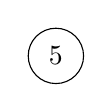
\begin{tikzpicture}

\node [shape = circle, minimum size = 2em, draw=black] at (0,0) {$5$};
\end{tikzpicture}
\end{center}
\end{figure}

A rank $n$ tree is a root node with $n$ children: the first a rank $n-1$ tree, the second a rank $n-2$ child and so on. The value of each child node must be larger than that of the root node.

\begin{figure}[h]
\begin{center}
    \begin{tikzpicture}

\node [shape=circle, minimum size = 2em, draw=black] (v1) at (0,0) {$3$};
\node [shape=circle, minimum size = 2em, draw=black] (v2) at (0,-1.5) {$6$};
\draw  (v1) edge (v2);
\node at (0,1) {Rank 1};
\node at (4.5,1) {Rank 2};
\node [shape=circle, minimum size = 2em, draw=black] (v3) at (4.5,0) {$2$};
\node [shape=circle, minimum size = 2em, draw=black] (v6) at (4.5,-1.5) {$5$};
\node [shape=circle, minimum size = 2em, draw=black] (v4) at (3,-1.5) {$4$};
\node [shape=circle, minimum size = 2em, draw=black] (v5) at (3,-3) {$7$};
\draw  (v3) edge (v4);
\draw  (v4) edge (v5);
\draw  (v3) edge (v6);
\node [shape=circle, minimum size = 2em, draw=black] (v7) at (11.5,0) {$3$};
\node [shape=circle, minimum size = 2em, draw=black] (v8) at (11.5,-1.5) {$9$};
\node [shape=circle, minimum size = 2em, draw=black] (v9) at (10,-1.5) {$6$};
\node [shape=circle, minimum size = 2em, draw=black] (v11) at (8.5,-1.5) {$7$};
\node [shape=circle, minimum size = 2em, draw=black] (v10) at (10,-3) {$7$};
\node [shape=circle, minimum size = 2em, draw=black] (v12) at (8.5,-3) {$9$};
\node [shape=circle, minimum size = 2em, draw=black] (v13) at (7,-3) {$9$};
\node [shape=circle, minimum size = 2em, draw=black] (v14) at (7,-4.5) {$9$};
\draw  (v7) edge (v8);
\draw  (v7) edge (v9);
\draw  (v9) edge (v10);
\draw  (v7) edge (v11);
\draw  (v11) edge (v12);
\draw  (v11) edge (v13);
\draw  (v13) edge (v14);
\node at (11.5,1) {Rank 3};
\end{tikzpicture}
\end{center}
\caption{Binomial trees of higher ranks}
\label{fig:binomial:rankn}
\end{figure}

We can join (or link) two trees of the same rank quickly by comparing their root nodes. The tree with the larger root becomes a child of the tree with the smaller one, increasing the rank of the new tree by one (\autoref{fig:binomial:merge}).

\begin{figure}[h]
\begin{center}
    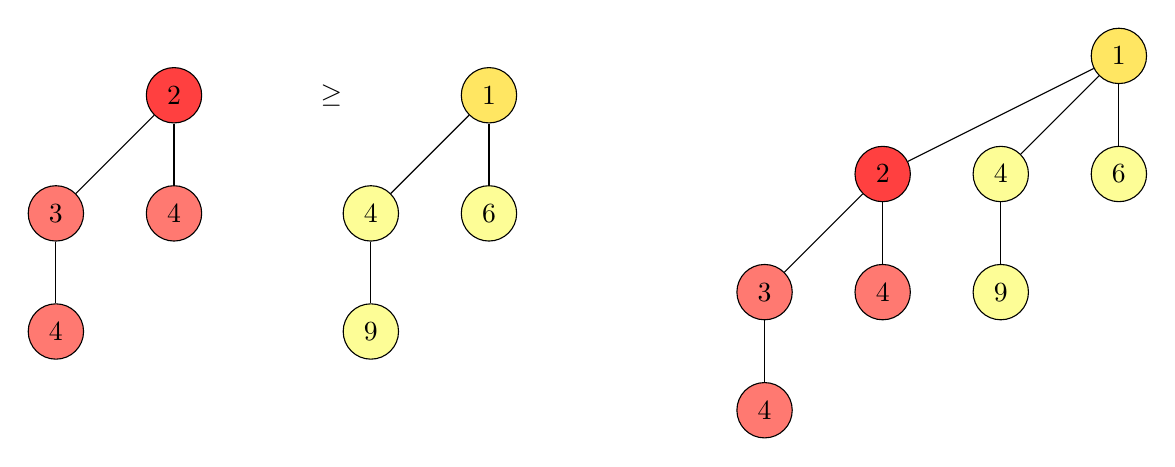
\begin{tikzpicture}
\definecolor{pastel-red}{HTML}{FF7971}
\definecolor{pastel-yellow}{HTML}{FDFD96}
\definecolor{sat-yellow}{HTML}{FFE662}
\definecolor{sat-red}{HTML}{FF4040}

\node [shape = circle, minimum size = 2em, draw = black, fill = sat-red] (v1) at (0,0) {$2$};
\node [shape = circle, minimum size = 2em, draw = black, fill = pastel-red] (v2) at (0,-1.5) {$4$};
\node [shape = circle, minimum size = 2em, draw = black, fill = pastel-red] (v3) at (-1.5,-1.5) {$3$};
\node [shape = circle, minimum size = 2em, draw = black, fill = pastel-red] (v4) at (-1.5,-3) {$4$};
\node [shape = circle, minimum size = 2em, draw = black, fill = sat-yellow] (v5) at (4,0) {$1$};
\node [shape = circle, minimum size = 2em, draw = black, fill = pastel-yellow] (v6) at (4,-1.5) {$6$};
\node [shape = circle, minimum size = 2em, draw = black, fill = pastel-yellow] (v7) at (2.5,-1.5) {$4$};
\node [shape = circle, minimum size = 2em, draw = black, fill = pastel-yellow] (v8) at (2.5,-3) {$9$};
\draw  (v1) edge (v2);
\draw  (v1) edge (v3);
\draw  (v3) edge (v4);
\draw  (v5) edge (v6);
\draw  (v5) edge (v7);
\draw  (v7) edge (v8);
\node at (2,0) {$\geq$};
\node at (6,-1.5) {$\implies$};


\node [shape = circle, minimum size = 2em, draw = black, fill = sat-red] (v21) at (9,-1) {$2$};
\node [shape = circle, minimum size = 2em, draw = black, fill = pastel-red] (v22) at (9,-2.5) {$4$};
\node [shape = circle, minimum size = 2em, draw = black, fill = pastel-red] (v23) at (7.5,-2.5) {$3$};
\node [shape = circle, minimum size = 2em, draw = black, fill = pastel-red] (v24) at (7.5,-4) {$4$};
\node [shape = circle, minimum size = 2em, draw = black, fill = sat-yellow] (v25) at (12,0.5) {$1$};
\node [shape = circle, minimum size = 2em, draw = black, fill = pastel-yellow] (v26) at (12,-1) {$6$};
\node [shape = circle, minimum size = 2em, draw = black, fill = pastel-yellow] (v27) at (10.5,-1) {$4$};
\node [shape = circle, minimum size = 2em, draw = black, fill = pastel-yellow] (v28) at (10.5,-2.5) {$9$};
\draw  (v25) edge (v26);
\draw  (v25) edge (v27);
\draw  (v27) edge (v28);
\draw  (v25) edge (v21);
\draw  (v21) edge (v22);
\draw  (v21) edge (v23);
\draw  (v24) edge (v23);
\end{tikzpicture}
\end{center}
\caption{Merging two binomial trees}
\label{fig:binomial:merge}
\end{figure}

Using these trees, we can now construct a binomial heap capable of storing any number of elements. We model a heap as a list of binomial trees of strictly increasing rank. A heap with $n$ elements has at most $1 + \lfloor \log_2 n \rfloor$ elements: The largest tree in this heap has rank $\lfloor \log_2 n \rfloor$ and then there can be only $\lfloor \log_2 n \rfloor$ trees with a smaller rank.

To find the minimum element, we iterate over all trees in the heap, finding the minimum among their root elements. Since there are only $\log n$ trees, this runs in $\mathcal O(\log n)$.

To insert an element into a heap, we create a rank zero tree containing just that element. Then we see if the heap contains a rank zero tree. If not, we can simply add the tree to the heap. Otherwise, we merge the two trees and repeat the process with the resulting rank one tree. This takes $k$ steps in total, where $k$ is the first rank for which no tree exists in the heap, $\mathcal O(\log n)$ in the worst case. However, we can show that the amortized runtime of an insert is constant:

Let $h$ be a heap. We define $\varphi(h)$ as the number of trees in the heap. Let $h' = insert x h$ the result of inserting an element $x$ into $h$ and $k$ the minimum rank for which $h$ does not contain a tree. Then $t(insert(x, h)) = k$ and $t_{am}(insert(x, h)) = k - \varphi(h) + \varphi(insert(x, h))$. Observe that the first $k$ trees of $h$ are removed after insertion because they are merged with the new tree. Instead, a new tree of rank $k$ is added. This means that $\varphi(insert(x, h)) = \varphi(h) - k + 1$ and thus $t_{am}(insert(x, h)) = 1$. A sequence of $n$ insert operations on an empty tree therefore has total amortized runtime $n$, so a single operation runs in amortized time $\mathcal O(1)$.

We can also merge two heaps in $\mathcal O(\log \max(k_1, k_2)$ where $k_1$ and $k_2$ are the number of elements in either heap. Starting at rank zero, we see if the two heaps both contain a tree of that rank. If not, we simply copy the tree of the heap that does, or leave the slot empty if neither does. If both heaps contain a tree, we merge the two and insert the result into the result heap at rank one. We then continue with the next rank. Observe that after merging at rank $n$, we will have filled at most the rank $(n+1)$ slot of the tree. If both trees contain a rank $n$ tree, we merge them into a rank $(n+1)$ tree and insert that. If only one heap does and the result also contains a rank $n$ tree from the previous merge step, we merge these two into a rank $(n+1)$ tree. Otherwise, we insert the single rank $n$ tree into the result. Each individual merge step runs in time $\mathcal O(1)$, and therefore the full merge runs in time $\mathcal O(\log \max(k_1, k_2))$.

Finally, we can remove the minimum element from a heap in time $\mathcal O(\log n)$. We find the minimum element as before. This time, we remove this tree in its entirety from the heap. This still leaves us with a valid heap. Since the child elements of a tree of rank $n$ form trees of rank $0$ to $n-1$, we can consider these child elements a heap in their own right. We therefore merge the child elements of the removed tree back into the main heap. Finding the minimum tree takes time $\mathcal O(\log n)$ and since the size of the heap after removing a tree and the size of the heap formed by the children of a tree are both less than the size of the original heap, the merge completes in time $\mathcal O(\log n)$ as well.

\section{Implementation}
With the theory out of the way, let us now consider how to implement this in our framework for amortized analysis.

A descending list of a type indexed by the natural numbers is a list where the last element is indexed by zero and each preceding element is indexed one higher. A binomial tree over a set $A$ is than either a leaf of rank zero, containing just a single element of $A$, or a node of rank $l+1$ containing an element of $A$ and a descending list of binomial trees from $l$ to zero.

\begin{lstlisting}[caption={Definition of a binomial tree},label={lst:binomial:tree},emph={DescList,BinomialTree,Leaf,Node}]
data DescList (A : bNat -> Set a) : bNat -> Set a where
    D[_] : A 0 -> DescList A 0
    _D::_ : A (suc l) -> DescList A l -> DescList A (suc l)

data BinomialTree (A : Set a) : bNat -> Set a where
    Leaf : A -> BinomialTree A 0
    Node :  A
         -> DescList (BinomialTree A) l
         -> BinomialTree A (suc l)

tSize : BinomialTree A l -> bNat
tSize {l = l} _ = 2 ^ l

tVal : BinomialTree A l -> A
tVal (Leaf x) = x
tVal (Node x _) = x
\end{lstlisting}

We can merge two trees of equal rank in constant time:

\begin{lstlisting}[caption={Merging two trees},label={lst:binomial:link},emph={link,Leaf,Node,if,then,else}]
link :  BinomialTree A l
     -> BinomialTree A l
     -> DecTree A (BinomialTree A (suc l)) 1
link (Leaf l) (Leaf r) = if l ≤? r
                         then return (Node l $ D[ Leaf r ])
                         else return (Node r $ D[ Leaf l ])
link l@(Node x xs) r@(Node y ys) =
                         if x ≤? y
                         then return (Node x $ r D:: xs)
                         else return (Node y $ l D:: ys)
\end{lstlisting}

A heap is represented as a contiguous list of binomial heaps or empty slots. It's indexed by two natural numbers: The minimum rank contained in the list and the total number of elements stores in the heap. The number of entries of a heap is the number of trees contained in it.

An empty heap can have any minimum rank and contains an element. An empty entry extends a heap with minimum rank $l+1$ to one with minimum rank $l$. An entry combines a tree of rank $l$ with a heap with minimum rank $l+1$ and $acc$ items into a heap of minimum rank $l$ and $2^l + acc$ items.

\begin{lstlisting}[caption={Definition of a binomial heap},label={lst:binomial:heap},emph={SparseTreeList,empty,entry,BinomialTree,entries}]
data SparseTreeList (A : Set a) : bNat -> bNat -> Set a where
    []        :  SparseTreeList A l 0
    empty::   :  SparseTreeList A (suc l) acc
              -> SparseTreeList A l acc
    entry_::_ :  {l acc acc' : bNat}
              -> {acc'\equiv2^l+acc : acc' \equiv 2 ^ l + acc}
              -> BinomialTree A l
              -> SparseTreeList A (suc l) acc
              -> SparseTreeList A l acc'


ts-acc : SparseTreeList A l acc -> bNat
ts-acc {acc = acc} _ = acc

entries : SparseTreeList A l acc -> bNat
entries [] = 0
entries (empty:: ts) = entries ts
entries (entry _ :: ts) = 1 + entries ts
\end{lstlisting}

For completeness sake we prove that the number of entries of a heap are bounded by the logarithm of total elements stored. As usual with long purely-mathematical proofs we omit the proof body here.

\begin{lstlisting}[caption={The length of a heap is bounded},label={lst:binomial:bounded},emph={SparseTreeList, entries}]
len\leq\lfloorlog\_2acc\rfloor :  (ts : SparseTreeList A l acc)
              -> entries ts \leq 1+\lfloorlog\_2 acc \rfloor
\end{lstlisting}

We can now provided \texttt{Amortized} declarations for a heap. We have two: One for heaps over a type $A$ and one for heaps over a type $A$ with minimum rank $0$.

\begin{lstlisting}[caption={Amortized declaration},label={lst:binomial:amortized},emph={tlist,amortized,Amortized}]
tlist-amortized0 :  (A : Set a)
                 -> Amortized (SparseTreeList A 0)
Amortized.i\_0        (tlist-amortized0 A) = 0
Amortized.initial   (tlist-amortized0 A) = []
Amortized.potential (tlist-amortized0 A) = entries
Amortized.init\equiv0    (tlist-amortized0 A) = refl

tlist-amortized' :  (A : Set a)
                 -> Amortized1 (SparseTreeList A)
Amortized1.i\_0        (tlist-amortized' A)   = 0
Amortized1.initial   (tlist-amortized' A) l = []
Amortized1.potential (tlist-amortized' A)   = entries
Amortized1.init\equiv0    (tlist-amortized' A) l =
        \leq-antisym (len\leq\lfloorlog\_2acc\rfloor
            (Amortized1.initial (tlist-amortized' A) l))
        z\leqn
\end{lstlisting}

We implement insertion into a heap where the minimum rank of the heap matches the rank of the inserted tree since this is sufficient for insertion of single elements into a heap with minimum rank zero. If the heap is empty or the rank $n$ slot is free, this means simply slotting the tree at the right position. Otherwise, we merge the new and the present tree and insert them in the remainder of the heap.

\begin{lstlisting}[caption={Inserting into a heap},label={lst:binomial:insert},emph={BinomialTree,SparseTreeList,insertTList,empty,entry}]
insertTList\equiv :  BinomialTree A l
             -> (ts : SparseTreeList A l acc)
             -> DecTree A
                  (SparseTreeList A l (2 ^ l + acc))
                  (leadingEntries ts)
insertTList\equiv t [] = return $ entry t :: []
insertTList\equiv t (empty:: ts) = return $ entry t :: ts
insertTList\equiv t (entry t' :: ts) = do
    t-join <- link t t'
    tlist-dec-subst-acc
        (+-assoc (2 ^ l) (2 ^ l) acc') $
    empty:: <$> insertTList\equiv t-join ts
\end{lstlisting}

Now we can show that an insertion always takes amortized constant time.

\begin{lstlisting}[caption={Insertion runs in constant time},label={lst:binomial:constinsert},emph={tlist,insert,pot,invariant,empty,entry,BinomialTree,SparseTreeList,leadingEntries,entries,insertTList}]
tlist-insert-pot-invariant :
              (t : BinomialTree A l)
           -> (ts : SparseTreeList A l acc)
           -> leadingEntries ts \ominus entries ts
              \bZ.+ entries (reduce $ insertTList\equiv t ts)
              \equiv + 1
tlist-insert-pot-invariant t [] = refl
tlist-insert-pot-invariant t (empty:: ts) =
            0-a+suca\equiv1 (entries ts)
tlist-insert-pot-invariant t ts@(entry x :: ts') = begin
      leadingEntries ts
    \ominus entries ts
    \bZ.+ entries (reduce $ insertTList\equiv t ts)

            \equiv\langle {- einsert -} \rangle

      leadingEntries ts'
    \ominus entries ts'
    \bZ.+ entries (reduce $
                 insertTList\equiv (reduce $ link t x) ts')

            \equiv\langle {- induction on (link t x), ts' -} \rangle

    + 1  \qed
  where
    open \equiv-Reasoning
    einsert : entries (reduce $ insertTList\equiv t ts)
            \equiv entries (reduce $ insertTList\equiv
                                     (reduce $ link t x) ts')
    einsert = begin
        entries (reduce (insertTList\equiv t ts))

            \equiv\langle {- bind-elim -} \rangle

        entries (reduce (empty:: <$>
                         insertTList\equiv (reduce (link t x)) ts'))

            \equiv\langle {- apply-elim -} \rangle

        entries (reduce $ insertTList\equiv
                            (reduce $ link t x) ts')

            \qed

\end{lstlisting}

And use this to show that performing $n$ insertions into an empty list runs in $\mathcal O(n)$.

\begin{lstlisting}[caption={$n$ inserts in linear time},label={lst:binomial:ins-in-linear-time},emph={tlist,insert,inserts,n,in,linear,time,insertTList,am,leadingEntries,potential}]
tlist-n-inserts : Vec A n -> Am (tlist-amortized0 A) A
tlist-n-inserts zero Vec.[] = lift
tlist-n-inserts (suc n) (x :: xs) = Am.step
                (tlist-n-inserts n xs)
                (\lambda ts -> insertTList\equiv (Leaf x) ts)

tlist-insert-in-linear-time :
                   (xs : Vec A n)
                -> atime-full (tlist-n-inserts xs) ≡ + n
tlist-insert-in-linear-time Vec.[] = refl
tlist-insert-in-linear-time (x :: xs) =
    let n-1-inserts = tlist-n-inserts xs in
    let n-inserts = tlist-n-inserts (x :: xs) in begin

        atime-full n-1-inserts
        \bZ.+ (leadingEntries (am-eval n-1-inserts)
             \ominus   am-potential n-1-inserts
             \bZ.+ am-potential n-inserts)

            \equiv\langle {- induction -} \rangle

        + n-1 \bZ.+ (leadingEntries (am-eval n-1-inserts)
                   \ominus   am-potential n-1-inserts
                   \bZ.+ am-potential n-inserts)

            \equiv\langle {- tlist-insert-pot-invariant -} \rangle

        + (n-1 + 1)  \qed
  where
    open ≡-Reasoning
\end{lstlisting}

In a similar vein, we can implement the remaining operations of a binomial heap: Merging two heaps, finding the minimum element and building on top of that, removing the minimum element from the heap. We list just there function signatures and omit the bodies for brevity's sake.

\begin{lstlisting}[caption={Remaining heap operations},label={lst:binomial:remaining},emph={SparseTreeList,tListMergeAm,merge,in,log,time,findMin,deleteMin}]
tListMergeAm :  (left : SparseTreeList A l acc)
             -> (right : SparseTreeList A l' acc')
             -> Am1 (tlist-amortized' A) A (l \lub l')

merge-in-log-time :  (left : SparseTreeList A l acc)
                  -> (right : SparseTreeList A l' acc')
                  -> atime-full1 (tListMergeAm left right) \
                     \bZ.\leq 2 * 1+\lfloorlog\_2 acc \lub acc' \rfloor

findMin :  SparseTreeList A l (suc acc)
        -> DecTree A A 1+\lfloorlog\_2 (suc acc) \rfloor

deleteMin :  (ts : SparseTreeList A l (suc acc))
          -> Am1 (tlist-amortized' A) A 0


deleteMin-in-log-time :  (ts : SparseTreeList A l (suc acc))
                      -> atime-full1 (deleteMin ts)
                         \bZ.\leq + 3 * 1+\lfloorlog\_2 suc acc \rfloor

\end{lstlisting}